% InterMoBA — APBC2026 (MDPI) supplementary materials (placeholder)
% =========================================================================
% This file is the **independent supplementary PDF** required by MDPI.
% Final submission: zip this directory into a single .zip and upload
% alongside the main manuscript on the MDPI submission portal.
% =========================================================================
\documentclass[11pt,a4paper]{article}
\usepackage[utf8]{inputenc}
\usepackage[T1]{fontenc}
\usepackage[margin=2.5cm]{geometry}
\usepackage{graphicx}
\usepackage{caption}
\usepackage{lineno}
\usepackage{fancyhdr}
\usepackage[hidelinks]{hyperref}

\linenumbers
\pagestyle{fancy}
\fancyhf{}
\fancyfoot[L]{\small APBC2026 --- Supplementary Materials}
\fancyfoot[R]{\thepage}
\renewcommand{\headrulewidth}{0pt}

\captionsetup{labelfont=bf,labelsep=period,justification=raggedright,singlelinecheck=false,skip=0pt}

\title{Supplementary Materials for InterMoBA}
\author{}
\date{}

\begin{document}
\maketitle
\thispagestyle{fancy}

\section*{Overview}
% TODO: short overview of supplementary materials

% Figure S1 (uses shared fig1.png)
\begin{figure}[htbp]
    \centering
    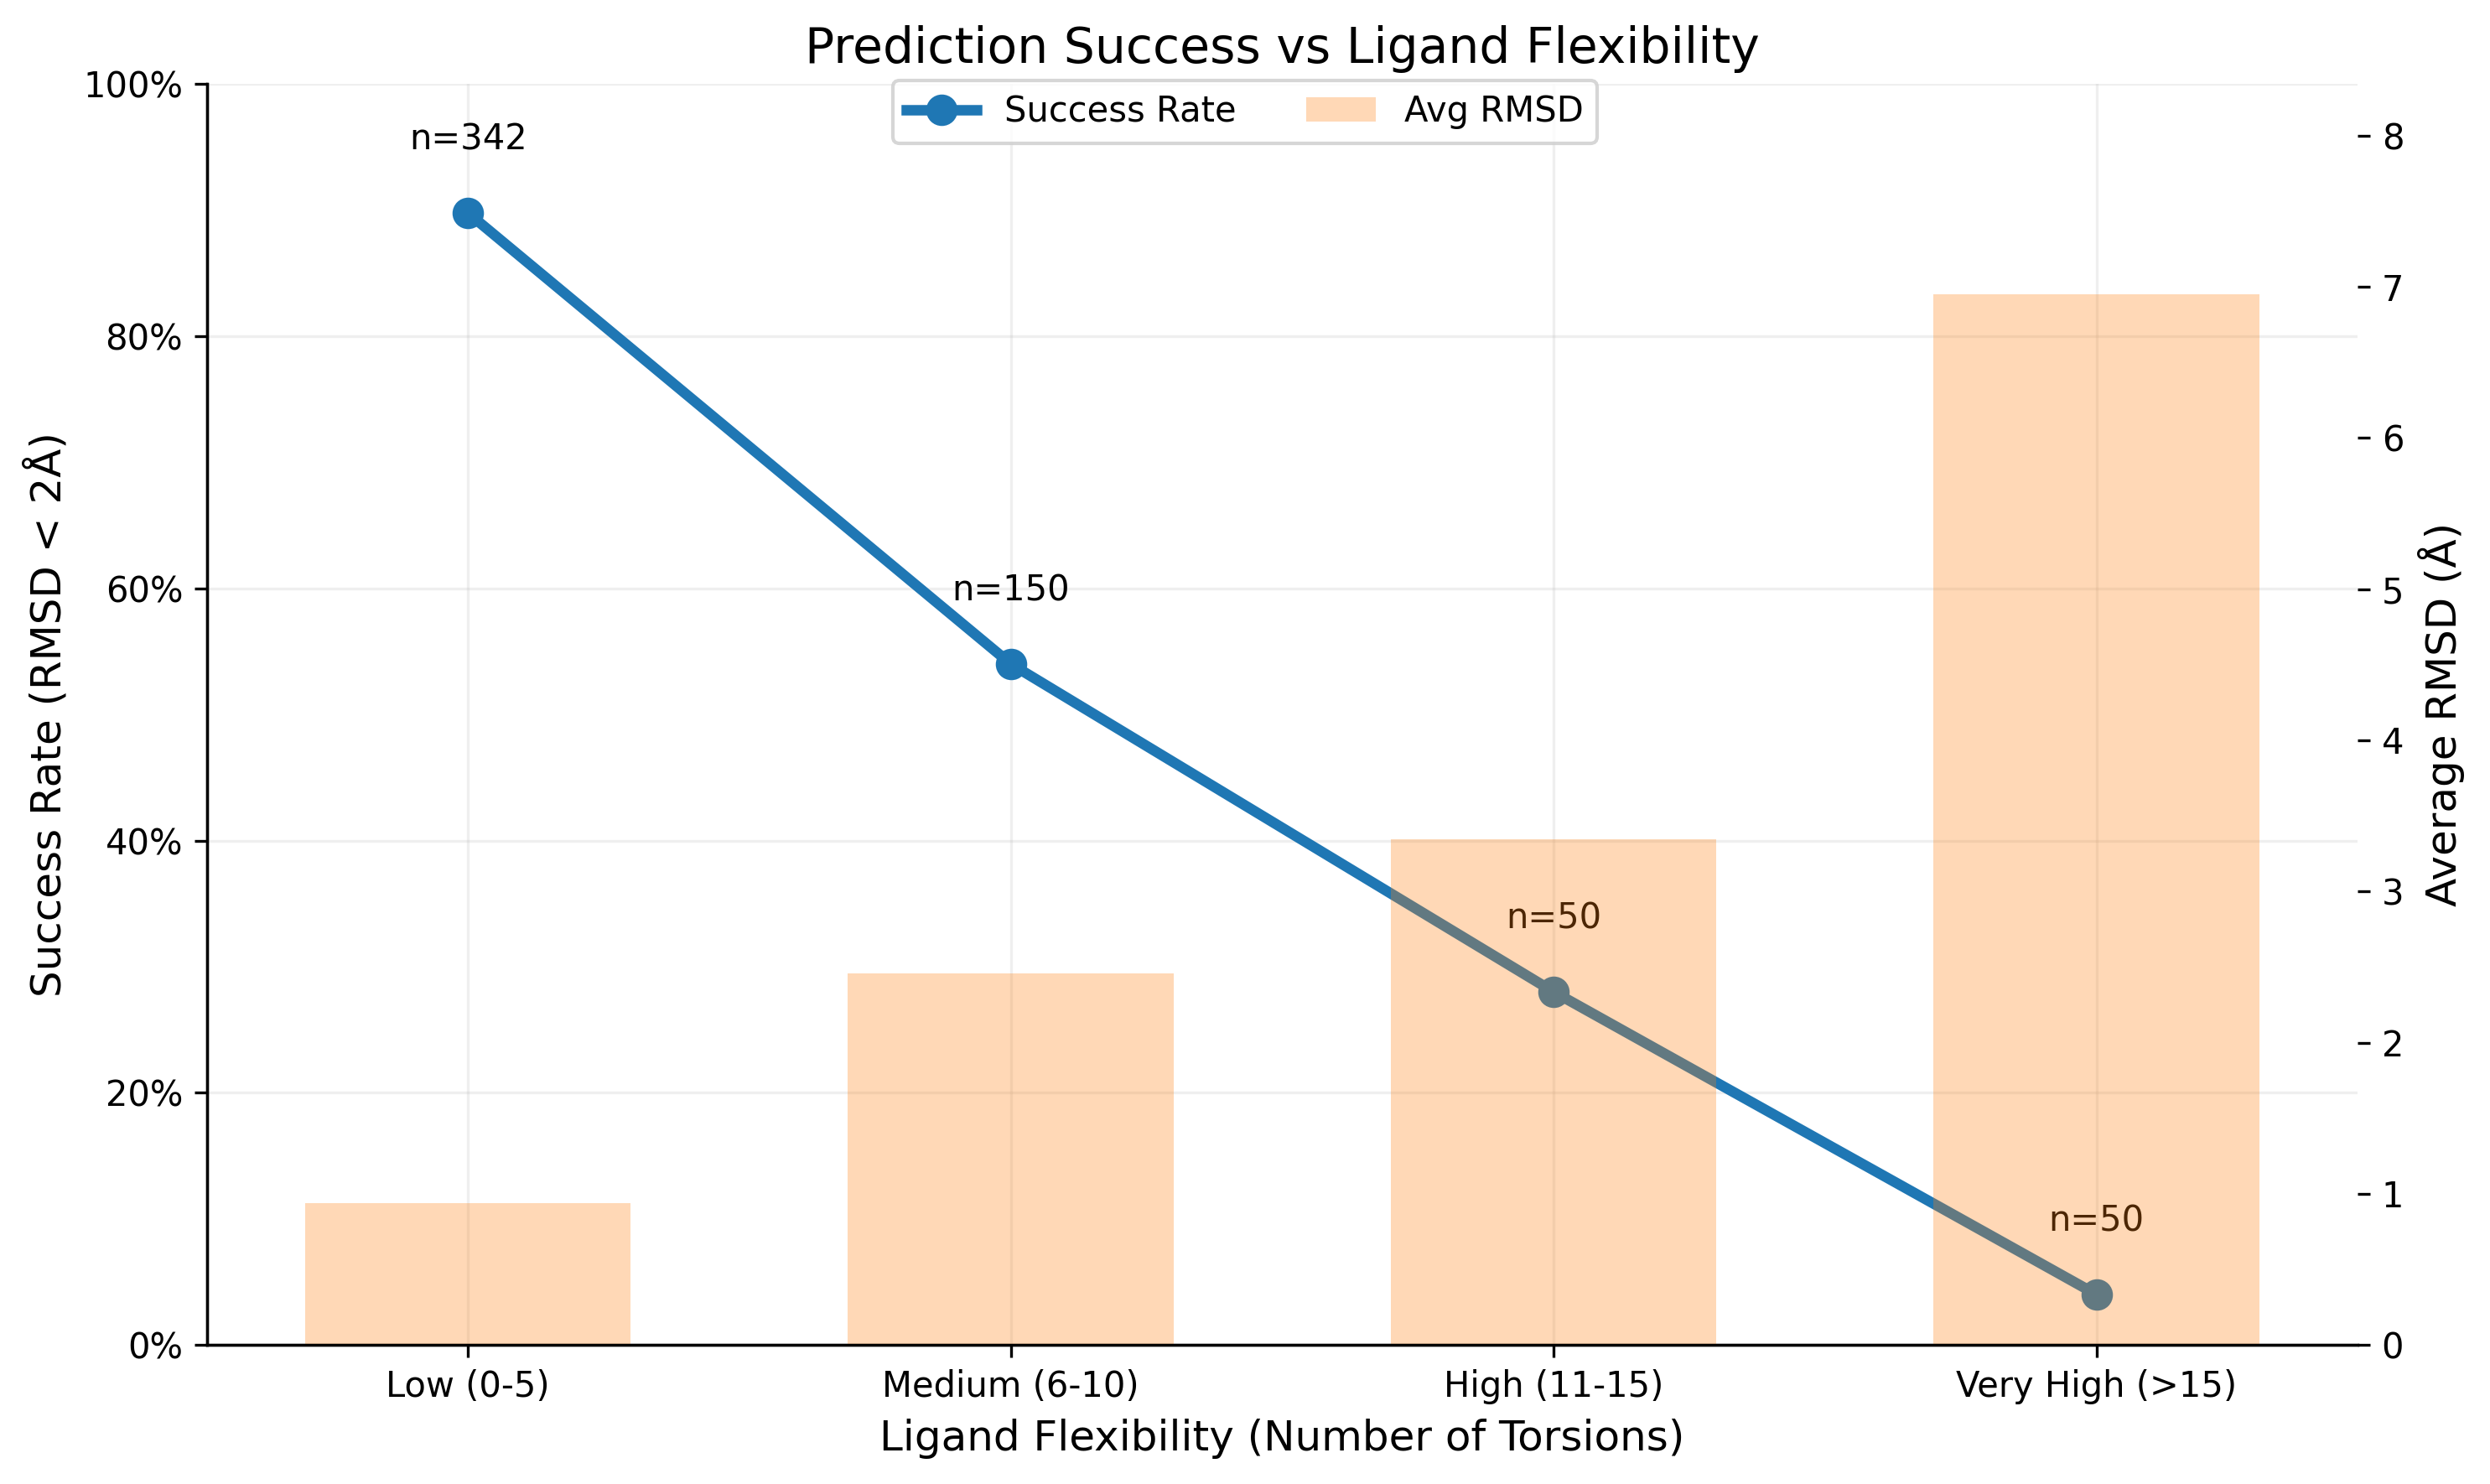
\includegraphics[width=0.8\textwidth]{figures/1.png}
    \caption{Correlation analysis between ligand flexibility and prediction success rate.}
\end{figure}

% Figure S2
\begin{figure}[htbp]
    \centering
    \includegraphics[width=\textwidth]{figures/2.png}
    \caption{Top-ranked pose RMSD vs.\ lower-ranked poses across 12 complexes.}
\end{figure}

% ... append S3..S15, S22, S88, S99, S1010, S1212, S1313, S1414, S1515 here

\end{document}
